\subsection{Osservabili stellari}

\begin{frame}<1>[label=noinside]{Modello stellare}{Come indagare la fisica interna a una stella?}

\onslide<1->\begin{block}{Osservabili stellari:}
$L$, $M$, $R$, $T_e$, $(\frac{Z}{X})_{ph}$, $g_{ph}$.
\end{block}

\onslide<1->\begin{block}{Informazioni sulla struttura interna?} Condizione di equilibrio idrostatico
\end{block}

%Teorema Vogt-Russel: $X_i(r)$, $M$ \pause equilibrio (idrostatico/termico) determinano struttura stellare .
%\pause

\onslide<1->\begin{block}{Modello stellare: diagramma di \hr{}.}
\end{block}

\onslide<2->\begin{block}{Descrizione fisica interno stellare: parametri aggiuntivi}
Convezione, diffusione e sedimentazione elementi pesanti, equazione di stato, opacit\'a
\end{block}

\onslide<2->\begin{block}{Astrosismologia}
Restringo spazio parametri sistemi stellari lontani
\end{block}

\end{frame}


{ % all template changes are local to this group.
    \setbeamertemplate{navigation symbols}{}
    \begin{frame}[plain]{Diagramma di \hr{}}
        \begin{tikzpicture}[remember picture,overlay]
            \node[at=(current page.center)] {
                %\includegraphics[width=\paperwidth]{yourimage}
            };
        \end{tikzpicture}
     \end{frame}
}



\againframe<2>{noinside}


\section{Osservazioni}

\subsection{Fitting polinomiale: inversione ''1.5-D''.}

\begin{frame}<1>[label=noinside]{Modello stellare}{Come indagare la fisica interna a una stella?}



\onslide<1->\begin{block}{Rotazione superficiale}
\begin{equation*}
\frac{\Omega(\theta)}{2\pi}=\SI{451.5}{\nano\hertz}-\SI{65.3}{\nano\hertz}\cos^2{\theta}-\SI{66.7}{\nano\hertz}\cos^4{\theta}
\end{equation*}

\end{block}

\onslide<1->\begin{block}{Informazioni sulla struttura interna?} Condizione di equilibrio idrostatico
\end{block}

%Teorema Vogt-Russel: $X_i(r)$, $M$ \pause equilibrio (idrostatico/termico) determinano struttura stellare .
%\pause

\onslide<1->\begin{block}{Modello stellare: diagramma di \hr{}.}
\end{block}

\onslide<2->\begin{block}{Descrizione fisica interno stellare: parametri aggiuntivi}
Convezione, diffusione e sedimentazione elementi pesanti, equazione di stato, opacit\'a
\end{block}

\onslide<2->\begin{block}{Astrosismologia}
Restringo spazio parametri sistemi stellari lontani
\end{block}

\end{frame}


\subsection{Osservazione dello splitting in m: inversione ''2D''.}

\begin{figure}[!ht]
\centering
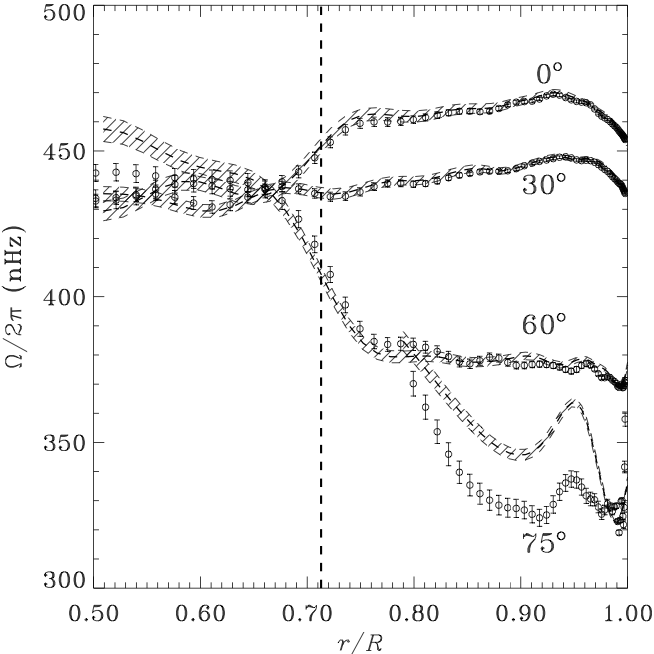
\includegraphics[keepaspectratio,width=0.8\textwidth]{invertedrotation}
\caption{Inversione della velocit\'a di rotazione a diverse latitudini. La linea verticale tratteggiata indica la base della zona convettiva. Da \cite{chr02helioseismology}.}
\end{figure}

Considero la correzione al primo ordine in $\Omega$. Il campo di velocit\'a rotazionale in coordinate sferiche \'e 
\begin{align}
&\vec{v_0}=(0,0,r\Omega\sin{\theta})=\vecp{\Omega}{r}\\
&\vec{\Omega(r,\theta)}=(\Omega(r,\theta)\cos{\theta},-\Omega(r,\theta)\sin{\theta},0)
\end{align}

In assenza di moti macroscopici il termine d'inerzia \'e $\rho_0\TDy{t}{\vec{v}}=\rho_0\PtwoDy{t}{\vec{\xi}}$, mentre in caso di rotazione si ha
\begin{equation}
\rho_0(\PDof{t}+\scap{v_0}{\nabla})^2\vec{\xi}
\end{equation}

Considero il termine dovuto alla rotazione come una piccola correzione alle frequenze dei modi
\begin{align}
&\omega_{(l,m)}+\Delta\omega_{(l,m)}&\intertext{quindi l'equazione del moto al primo ordine nella perturbazione, con $\alpha=(l,m)$, \'e}\nonumber\\
&\rho_0(\omega_{\alpha}^2+2\omega_{\alpha}\Delta\omega_{\alpha})\vec{\xi}=\nabla P_1-\frac{\rho_1}{\rho_0}\nabla P_0+\rho_0\nabla\Phi_1+2i\omega_{\alpha}\rho_0(\scap{v_0}{\nabla})\vec{\xi}\\
&\intertext{da cui si deduce}\nonumber\\
&\Delta\omega_{\alpha}=\frac{i\int\rho_0\xi_{\alpha}^*(\scap{v_0}{\nabla})\xi_{\alpha}}{\int\rho_0\xi_{\alpha}^*\xi_{\alpha}}=\frac{-m\int\rho_0\Omega\xi_{\alpha}^*\xi_{\alpha}\,dV+i\int\rho_0\xi_{\alpha}^*(\vecp{\Omega}{\xi_{\alpha}})\,dV}{\int\rho_0\xi_{\alpha}^*\xi_{\alpha}}
\end{align}

Il problema di trovare $\Omega(r,\theta)$ dalla differenza $\Delta\omega_{\alpha}$ \'e lineare in $\Omega$ quindi $\Delta\omega_{\alpha}\propto\Omega$. Per determinare quindi la rotazione dobbiamo conoscere l'autovalore $\xi_{\alpha}$ dello stato imperturbato.

%Per rotazione puramente radiale $\Omega(r)$ la relazione tra lo splitting delle frequenze e la rotazione \'e
%\begin{equation}
%\Delta\omega_{\alpha}=-m\frac{\int_0^{\rsun{}}\rho_0\Omega\{|\xi_r-\xi_h|^2+[l(l+1)-2]|\xi_h|^2\}r^2\,dr}{\int_0^{\rsun{}}\rho_0\{|\xi_r|^2+l(l+1)|\xi_h|^2\}r^2\,dr}=\int_0^{\rsun{}}K_{\alpha}(r)\Omega(r)\,dr
%\end{equation}
%Any given $\Delta\omega_{\alpha}$ samples angular velocity in the depth range corresponding to $\xi_{\alpha}$.

La velocit\'a angolare contribuisce a $\Delta\omega_{\alpha}$ negli strati in cui $\xi_{\alpha}$ \'e apprezzabile. Nel caso di rotazione dipendente solo da r si ha che $\Delta\omega_{\alpha}$ \'e lineare in m: ho $2l+1$ frequenze equispaziate.

